\section{Introduction}
Observational sciences such as astronomy have long relied on computing
to extract scientific discoveries from measurements. Since
cause and effect cannot be studied directly with controlled experiments, expert analysis
of data is the only way that processes which cannot be interacted with can be
understood. 

This is true in the field of heliophysics whose goal is to understand the sun and its interactions with Earth and the solar system, including space weather. This field includes a number of sub-disciplines such as solar physics, ionospheric and magnetospheric physics. The only way to make significant progress in understanding the fundamental processes in this complex system requires that interconnections be made across traditional science disciplines. This is made difficult by the diversity of data sets involved. At the time of writing, NASA alone operates 18 missions with 24 spacecraft with 5 missions current under development as part of its Heliophysics Systems Observatory.  Software packages to analyze these datasets have generally been developed by the projects that designed and built the observatories through direct funding. These packages have provided some level of documentation and user support with various levels of quality. The result of this approach is a diverse and therefore difficult data environment to traverse. A common platform that addresses simple tasks, provides a standardize interface to data products, and encourages re-use of common functions can go a long way toward solving this problem. SunPy is a project which aims to solve this problem for the field of solar physics. 

The primary goal of the SunPy Project is to facilitate and promote the use and development of a community-led, free and open-source data-analysis software based on the scientific \python\footnote{\url{https://www.python.org/}} environment. To achieve that goal the project develops and maintains a core package (\sunpypkg) and supports an ecosystem of affiliated packages that provide additional functionality built on top of the core package. The project was formally founded in March of 2014. Development of the core package began three years earlier. Version 0.5, which was released on Jun 2014. was described in \citep{Community:2015cy}.

The project began as a community-led effort to organize and standardize existing functionality and also to provide a free and modern alternative to the existing SolarSoft (SSW, \citet{Freeland:1998we}) software package. While SSW is open source and freely available, it is primarily composed of source code for the Interactive Data Language (IDL), a proprietary data-analysis environment currently owned by Harris Geospatial Solutions. In addition, the development of SSW is not open to the community and is not version controlled.

The SunPy project has chosen \package{Python} to leverage the rich ecosystem of packages available for general scientific analysis. These include packages such as
\package{Numpy} which provides efficient multi-dimensional numerical array manipulation \citep{numpy} ; \package{scipy} which provides fundamental scientific functions such as for numerical integration and optimization\citep{scipy}; \package{Matplotlib} provides publication-ready 2D plotting \citep{matplotlib}, and finally \package{Pandas} provides data structures and analysis support with support for time series \citep{pandas}. These packages form the foundation of the scientific \python ecosystem. Together they represent $>$500,000 lines of code\footnote{As measured by cloc (\url{github.com/AlDanial/cloc})}. Significant packages have been built on top of these foundations. Of particular relevance to \sunpypkg is the \package{Astropy} package which provides common core functionality for astronomy \citep{astropy2018}. 

%NumPy 102906 LOC
%SciPy 139009 LOC
%matplotlib 98720 LOC
%pandas 212338 LOC
%astropy 151825 LOC

%The SunPy Project aims to develop and provide high-quality, maintainable and tested code paired with extensive documentation that follow current best practices in software development. 

%The core library sets a standard and example for other codes to follow.

%A description of the current affiliated packages can be found in Section~\ref{sec:affil_packages}.

\section{Project Organization \& Enhancement Proposals - Steven Christe}
The \sunpy project has defined a formal mechanism to define itself as well as to propose significant changes to the project or to the core package. These proposals are referred
to as referred \sunpy Enhancement Proposals (SEPs) and are modeled after the Python Enhancement Proposal process. SEPs are used to define the project, the leadership structure, decision-making mechanisms, as well as propose new features for the \sunpypkg package. There are generally three types of SEP. 
\begin{itemize}
    \item \textbf{Standard}: introduces and describes a new feature or changes to an existing feature (e.g. API change) and is meant to function as a high-level design document.
    \item \textbf{Process}: This type of SEP describes a new process or a change to an existing process in the management of the project. Examples include procedures, guidelines, changes to the decision-making process or management structure, and changes to the tools or environment.
    \item \textbf{Informational}: Provides information and does not introduce any new features or changes nor describes a new process.
\end{itemize}
The first two SEPs (SEP-0001 and SEP-0002) define themselves as well as the \sunpy project organization. They are version controlled and publicly available on \github\footnote{\url{https://github.com/sunpy/sunpy-SEP}}. The organization is designed similar to a non-profit with a board and an executive director. The board is composed of up to 10 community members who are elected by the board. The board also elects the executive director also referred to as the lead developer. The responsibilities of the lead developer include leading the developer community, providing user support, implementing new SEPs, developing and maintaing the core package, as well as support the development of affiliated packages. The lead developer is supported by a deputy as well as other volunteers from the developer community. Members of the board are elected to serve two year terms while the Lead Developer serves one year long terms. This choice of structure is enable significant community involvement in the leadership of the project.

As of the time of writing, there are a total of 8 SEPs. Some notables SEPs have lead to the adoption of physical units throughout the code base (SEP-0003), defined the affiliated package program (SEP-0004), standardized the use of coordinate and coordinate transformations (SEP-0005), and led to the adoption of a high precision scientific time format (SEP-0008).

\section{Support \& Sustainability}
The \sunpy project has not received any significant direct financial support for its work facilitating and promoting open-source and open development software including developing \sunpypkg. All development time, including the creation of supporting materials (e.g. documentation) and community and technical support has been donated to the project by individuals working in their free time or as part of their regular work duties. This situation is similar to that faced by the \astropy project \citep{PriceWhelan:2018ji}. The \sunpy project is actively searching for appropriate funding models to support long-term sustainability. The \sunpy project has the ability to accept financial contributions from institutions or individuals through the NumFOCUS organization.

\section{Development Model - NABIL}
The 
\verb|sunpy core| package is hosted online and all development is open to the community via 

\begin{figure}
\begin{tabular}{ccc}
  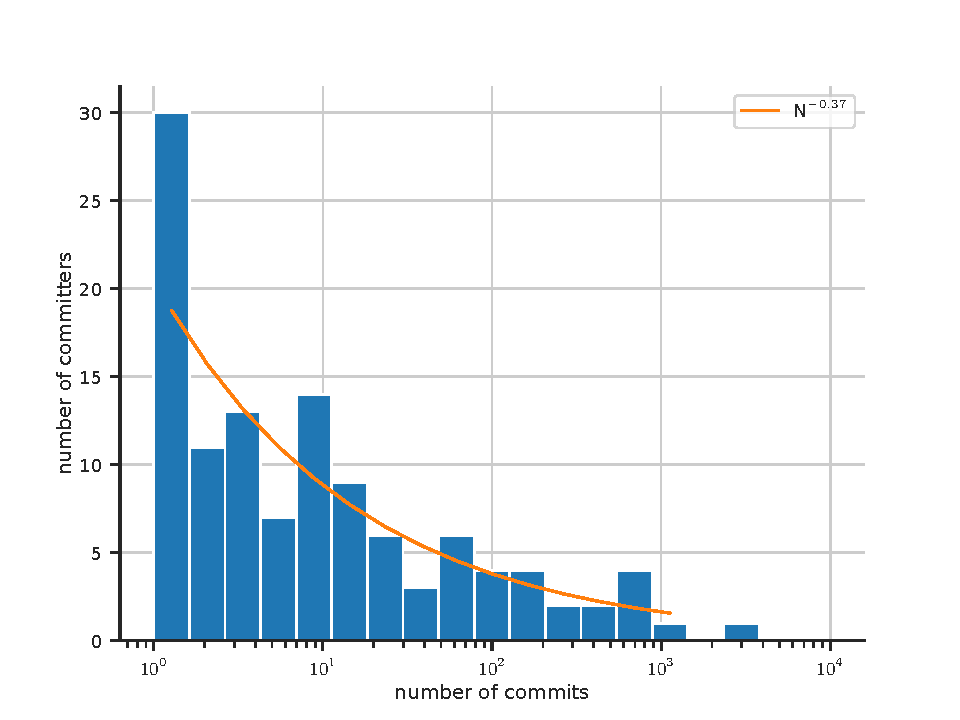
\includegraphics[width=55mm]{figures/busfactor_plot.pdf} &   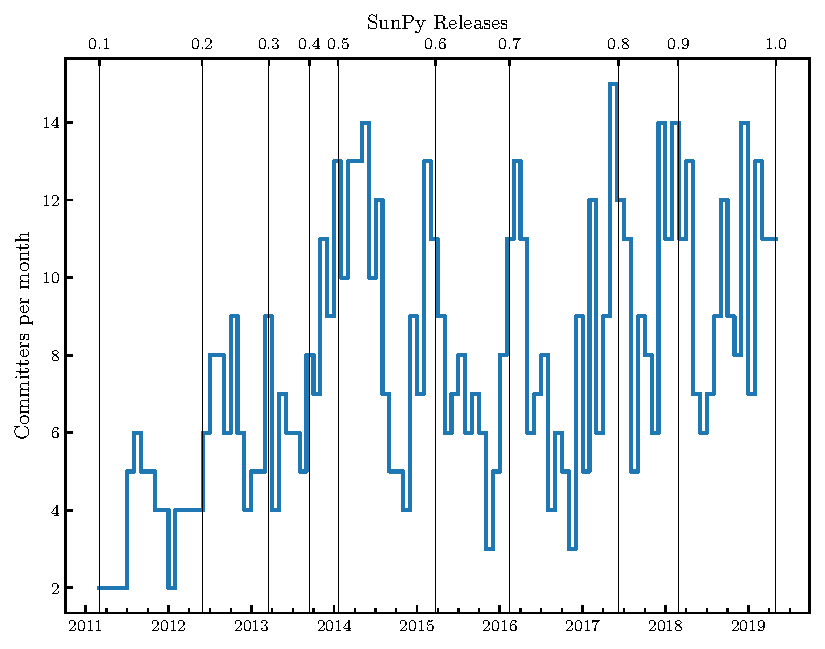
\includegraphics[width=55mm]{figures/committers_per_month_vs_time.pdf} &
  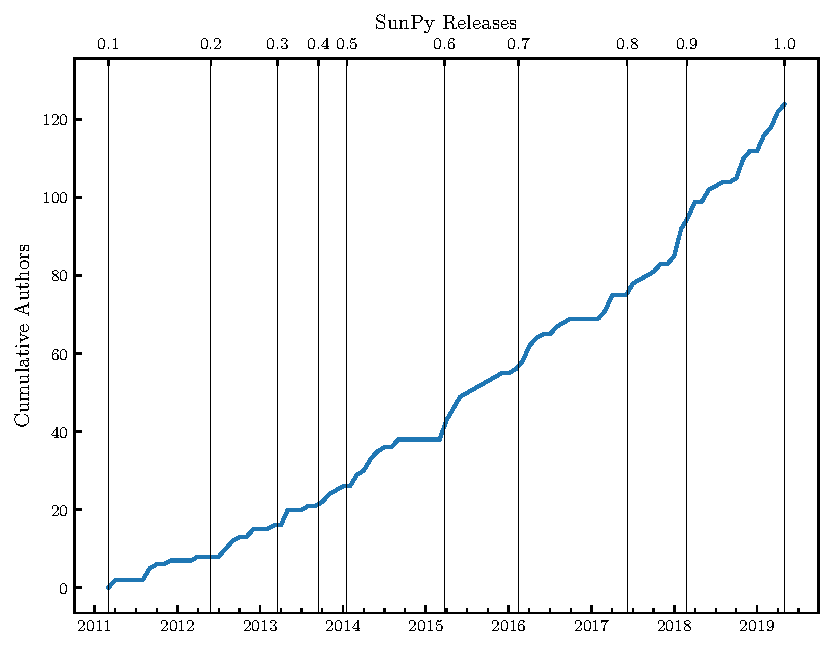
\includegraphics[width=55mm]{figures/cumulative_authors.pdf} \\
(a) first & (b) second & (c) third
\end{tabular}
\caption{caption}
\label{fig:image2}
\end{figure}

